\documentclass[12pt,a4paper]{report}
\usepackage[utf8]{inputenc}
\usepackage[francais]{babel}
\usepackage[T1]{fontenc}
\usepackage{amsmath}
\usepackage{amsfonts}
\usepackage{amssymb}
\usepackage{url}
\usepackage{ucs}
\usepackage{graphicx}
\usepackage{lmodern}
\usepackage{xcolor}
\usepackage[left=2cm,right=2cm,top=2cm,bottom=2cm]{geometry}
\author{Typhaine PL}
\setcounter{tocdepth}{1} 
\usepackage{lmodern}
\usepackage{fancyvrb}
\definecolor{Zgris}{rgb}{0.87,0.85,0.85}

% Pour avoir du code coloré
\usepackage{listings}
\lstset{
language=HTML,        % choix du langage
basicstyle=\ttfamily\footnotesize,       % taille de la police du code
keywordstyle=\ttfamily\bfseries\color{red},  %style des mots clefs
commentstyle=\ttfamily\slshape\color{darkgreen},  %style des commentaires
identifierstyle=  \ttfamily\color{blue},  %style des identificateurs
stringstyle= \ttfamily\color{green},  %style des chaines de caractères
showstringspaces=false,
numbers=left,                   % placer les numéros de lignes à gauche (left)
numberstyle=\footnotesize,        % taille de la police des numéros
numbersep=6pt,            % distance entre le code et sa numérotation
tabsize=4,
xleftmargin=17pt,
escapeinside={\%*}{*)},
breaklines=true,
breakatwhitespace=true,
string=[b]{'}
}

\newsavebox{\BBbox}
\newenvironment{DDbox}[1]{
\begin{lrbox}{\BBbox}\begin{minipage}{\linewidth}}
{\end{minipage}\end{lrbox}\noindent\colorbox{Zgris}{\usebox{\BBbox}} \\
[.5cm]}

\makeatletter
\def\clap#1{\hbox to 0pt{\hss #1\hss}}%
\def\ligne#1{%
\hbox to \hsize{%
\vbox{\centering #1}}}%
\def\haut#1#2#3{%
\hbox to \hsize{%
\rlap{\vtop{\raggedright #1}}%
\hss
\clap{\vtop{\centering #2}}%
\hss
\llap{\vtop{\raggedleft #3}}}}%
\def\bas#1#2#3{%
\hbox to \hsize{%
\rlap{\vbox{\raggedright #1}}%
\hss
\clap{\vbox{\centering #2}}%
\hss
\llap{\vbox{\raggedleft #3}}}}%
\def\maketitle{%
\thispagestyle{empty}\vbox to \vsize{%
\haut{}{\@blurb}{}
\vfill
\vspace{1cm}
\begin{flushleft}
\usefont{OT1}{ptm}{m}{n}
\huge \@title
\end{flushleft}
\par
\hrule height 4pt
\par
\begin{flushright}
\usefont{OT1}{phv}{m}{n}
\Large \@author
\par
\end{flushright}
\vspace{1cm}
\vfill
\begin{center}

\includegraphics[width=0.3\textwidth]{../Images/logo/logo.png}\\
\vspace{2cm}

\includegraphics[width=0.1\textwidth]{../Images/logounibdx.png}
\end{center}
\vfill
\bas{}{\@date}{}
}%
\cleardoublepage
}
\def\date#1{\def\@date{#1}}
\def\author#1{\def\@author{#1}}
\def\title#1{\def\@title{#1}}
\def\location#1{\def\@location{#1}}
\def\blurb#1{\def\@blurb{#1}}
\date{\today}
\author{}
\title{}
\location{}\blurb{}
\makeatother

\title{Conception d'un Projet de Recherche}
\author{\textsc{FR\`ECHE} Arnaud, \textsc{H\'ERIC\'E} Charlotte, \textsc{MOLA} Saraï,\\ \textsc{PAYSAN-LAFOSSE} Typhaine, \textsc{SANSEN} Joris}
\location{Bordeaux}
\blurb{%
Universités de Bordeaux\\
Master 2 BioInformatique
\textbf{}\\[1em]
\textsc{Marie \textsc{Beurton-Aimar}}
}%

\begin{document}
\maketitle

\chapter*{Résumé}
\addcontentsline{toc}{chapter}{Résumé}

Le logiciel \emph{regEfmtool} permet la modélisation de réseaux métaboliques et le calcul de mode élémentaires. Ce logiciel fonctionne sous environnement \emph{UNIX} uniquement en ligne de commande et nécessite plusieurs fichiers d'entrée au format texte. Ces derniers doivent être générés à la main et contiennent les informations sur ce réseaux. Sa prise en main n'est donc pas aisée pour un utilisateur ne possédant aucune connaissance en programmation.\\

Dans le cadre de l'UE Conception d'un Projet de Recherche du Master 2 BioInformatique, notre but était de réaliser une interface graphique (en langages Web) afin de pallier au manque d'ergonomie de \emph{regEfmtool}. A l'heure actuelle aucune méthode ne permet de générer les fichiers d'entrée de \emph{regEfmtool}, ni de le lancer sans ligne de commande.\\

Cette interface nommée \emph{WRET : WebRegEfmTool} permet de générer les fichiers nécessaires a l'utilisation de ce logiciel de modélisation sans avoir à l'installer  sur son système. Elle permet également la création de réseaux au format \emph{DAT} afin de lancer des simulations comparées sur le logiciel \emph{METATOOL}.

\tableofcontents
\listoffigures

\chapter*{Introduction}
\addcontentsline{toc}{chapter}{Introduction}

Intro ...

\chapter{Analyse}

%%%%%%%%%%%%%%%%%%%%%%%%%%%%%%
\section{Contexte}
%%%%%%%%%%%%%%%%%%%%%%%%%%%%%%

\subsection{Sujet}
Le métabolisme d'une cellule est un système complexe de transformations moléculaires et énergétiques qui se déroulent de manière ininterrompue dans la cellule et mettant en jeu un ensemble de réactions dites métaboliques. 
Ces réactions impliquent différents types de métabolites qui, suivant leurs positions dans la réaction, sont appelés substrats ou produits et catalysés par des enzymes.

La représentation visuelle des grandes fonctions métaboliques (glycolyse ou photosynthèse par exemple) sous la forme de réseaux pourrait être un outil précieux pour faciliter l'avancement des travaux des chercheurs. Cette modélisation de réactions permet de réaliser des requêtes complexes comme, par exemple, le calcul (et la prédiction) de tous les métabolites pouvant être générés à partir d'un ensemble de composés sources.

Quelques logiciels disponibles internationalement permettent de travailler et d'automatiser l'étude de ces réseaux, tout en proposant des fonctionnalités telles que le calcul des modes élémentaires de flux ou la recherche de \textit{minimal cut sets}\footnote{Un \textit{minimal cut sets}~\cite{mcs:url} (MCS) est un ensemble minimal (irréductible)de réactions dans le réseau dont l'activation va certainement conduire à une défaillance de certaines fonctions du réseau.}.  Cependant, ils peuvent être dépendants de logiciels non libres comme MATLAB ou alors ne pas avoir d'interface utilisateur conviviale, ce qui est le cas avec  \emph{regEfmtool} (logiciel sur lequel nous nous appuierons pour ce projet).

\subsection{Objectif}
Dans le cadre de cette U.E., il nous est demandé de créer un programme (package et documentation à fournir à la fin du projet) nous permettant d'approfondir ou d'apprendre un langage de programmation, et de réaliser une analyse critique du travail effectué. L'objectif de ce projet sera donc de réaliser une interface graphique du programme  \emph{regEfmtool} qui ne peut être utilisé, à l'heure actuelle, que par des commandes à l'aide d'une console. \\

Deux possibilités s'offraient à nous pour réaliser cette interface: nous avions le choix entre les technologies Web et le langage Java. Nous avons choisi de nous appuyer sur les technologies Web. En effet, beaucoup de programmes utilisent une interface de type site Web leur permettant d'une part de créer une interface graphique conviviale, feuilles de style, tout en permettant une certaine modularité. 
\pagebreak
%%%%%%%%%%%%%%%%%%%%%%%%%%%%%%
\chapter{État de l'existant}
%%%%%%%%%%%%%%%%%%%%%%%%%%%%%%

\section{Efmtool}
Efmtool~\cite{efmtool:url} calcule les modes élémentaires de flux de réseaux métaboliques. Il est implémenté en Java et a été intégré à MATLAB.\\
Il a été développé par Marco Terzer. La version courante est la 4.7.1 (Décembre 2009).

\section{\emph{RegEfmtool}}
\emph{RegEfmtool}~\cite{regefmtool2:url} est un outil informatique qui combine le calcul des modes élémentaires de flux et la régulation transcriptionnelle du réseau métabolique. Il a été développé, entre autres, par Christian Jungreuthmayer. Il a été créé afin d'accélérer le calcul de jeux complets de modes élémentaires de flux d'un réseau métabolique.\\
\emph{RegEfmtool} est une extension d'Efmtool qui prend en compte la régulation transcriptionnelle des réseaux pour le calcul des modes élémentaires de flux.\\
La prise en compte de la régulation des gènes réduit de façon importante le nombre de solutions et permet d'éliminer constamment les modes qui ne peuvent exister biologiquement pendant et après le processus de calcul. Elle permet aussi de réduire considérablement le coût du calcul.\\
L'installation et l'utilisation de \emph{regEfmtool} a été exclusivement testée sous Linux. Elle pourrait cependant fonctionner sous d'autres systèmes d'exploitation puisqu'il s'agit d'un programme Java. Il n'existe pas d'interface graphique de cette application, elle s'exécute donc en lignes de commandes via le terminal.
La version courante de \emph{RegEfmtool} est la 2.0 (Août 2012).

\section{METATOOL} 
METATOOL~\cite{metatool:url} est un programme écrit en C développé de 1998 à 2000 par Thomas Pfeiffer (Berlin) en coopération avec Juan Carlos Nuno (Madrid), Stefan Schuster (Berlin) et Ferdinand Moldenhauer (Berlin).\\
Il sert à étudier la structure des réseaux métaboliques à partir d'équations de réactions stœchiométriques et permet notamment de calculer les modes élémentaires.\\
Les premières versions de METATOOL (jusqu'à la 4.9) ont été développées en C. Aujourd'hui, nous trouvons aussi une version de METATOOL en C++ mais cette version n'est pas au point. La dernière version, 4.9, est assez performante sur les petits réseaux métaboliques, mais possède de gros problèmes de gestion de mémoire et de rapidité lors de calculs sur de grands réseaux.
Dans la version actuelle (5.1) l'exécutable est désormais un module de MATLAB 7 et GNU 3.0 Octave, il se présente sous la forme d'un ensemble de fichiers scripts de MATLAB.\\

Les paramètres donnés en entrée pour le bon fonctionnement du logiciel METATOOL sont les suivants:
\begin{enumerate}
\item la liste des réactions réversibles, ainsi que celle des réactions irréversibles, avec le nom des réactions,
\item la liste des métabolites internes et externes impliqués dans les réactions,
\item les équations réactionnelles se trouvant dans la section.
\end{enumerate}
Le tout est rassemblé dans un fichier avec l'extension \textit{.dat}\\

A la fin de son exécution, METATOOL a généré un fichier avec l'extension \textit{.out} dans lequel se trouvent les résultats. Dans les versions de METATOOL écrites en C, le fichier de sortie contient l'ensemble des résultats sous forme de matrices, ainsi que des bilans qui permettent de décrire le réseau d'étude.\\
Les versions de METATOOL écrites en MATLAB produisent des résultats similaires en terme de calcul des matrices des modes élémentaires mais les résultats sont disposés différemment dans le fichier de sortie.

\section{CellNetAnalyzer}
CellNetAnalyzer~\cite{cna:url} est un package de MATLAB (écrit en \textsc{C}) qui fourni un environnement compréhensible et convivial pour l'utilisateur et qui permet une analyse fonctionnelle et structurelle de réseaux biochimiques. Il a été développé à l'institut Max Planck de Magdeburg par Steffen Klamt (depuis 2000) et Axel von Kamp (depuis 2007) notamment.\\
CellNetAnalyzer fourni une importante collection d'outils et d'algorithmes pour l'analyse structurelle de réseaux.\\
C'est un programme gratuit pour une utilisation académique. Pour l'exécuter, il faut avoir installé MATLAB 7.0 ou une version ultérieure qui demande une licence. Il peut être utilisé sur Linux, Windows XP ou Mac.\\
Pour l'étude des modes élémentaires, CellNetAnalyzer fait appel à METATOOL via le logiciel MEX qui sert d'interface. MEX permet à MATLAB d'appeler tout logiciel \textsc{C} externe pour compléter les outils qu'il possède.

\section{Yana}
YANA~\cite{yana:url} est un logiciel libre, écrit en JAVA, utilisant METATOOL pour l'étude
des voies métaboliques. Il contient le logiciel METATOOL dans sa structure interne. \\
YANAsquare~\cite{yanasq:url} sert de façade et de sortie à METATOOL 6 tout en implémentant d'autres fonctions d'analyses du métabolisme (ex: quantification de l'activité enzymatique des réactions).\\ YANA s'occupe de l'entrée des données vers METATOOL puis il effectue une analyse syntaxique du fichier \textit{.out} pour afficher les résultats sur une interface graphique et effectuer des analyses complémentaires sur ceux-ci.

\section{Acom}
ACoM~\cite{acom:url} fonctionne à partir des fichiers de sortie de METATOOL. Il permet une classification automatiques des modes élémentaires en fonction d'une taille minimale et d'un seuil de similarité. Il est surtout utilisé pour l'analyse des réseaux de grandes tailles où la manipulation des données à la main est laborieuse. ACoM est un programme
C utilisable uniquement en mode console.

\section{JACoMode}
JACoMode est une interface Web permettant lancement d'ACoM via le Web. En plus d'obtenir les résultats d'ACoM, JACoMode traite ces résultats pour obtenir d'autres résultats statistiques sur les modes élémentaires.

\section{Langages}
Notre projet nécessite l'utilisation d'une interface Web, dans ce cadre il existe:
\begin{itemize}
\item Mod Perl combiné avec Apache\footnote{Apache HTTP Server} et CGI\footnote{CGI: Common Gateway Interface.} mais la technologie utilisée est à l'heure actuelle dépassée
\item Mod Python combiné avec Apache et CGI mais même remarque que précédemment
\item CL-WHO avec Hunchentoot\footnote{Hunchentoot HTTP Server} et ParenScript offre un bon environnement pour le développement Web
\item Java et ses applets\footnote{Applet Java: logiciel s'exécutant dans la fenêtre d'une navigateur Web (grâce à une machine virtuelle Java (JVM)), fournie aux utilisateurs sous la forme de bytecode Java.} apparaissent également comme un bon choix pour le développent Web
\item PHP couplé avec du JavaScript peut être un choix judicieux pour une application Web
\end{itemize}

Parmi les différents choix précédemment cités, deux sortent du lot: Java et PHP avec leurs bibliothèques.
\pagebreak
%%%%%%%%%%%%%%%%%%%%%%%%%%%%%%
\section{Analyse des besoins}
%%%%%%%%%%%%%%%%%%%%%%%%%%%%%%

\subsection{Besoins fonctionnels}

\subsubsection{Interface Homme Machine (IHM)}
L'interface Web que nous avons réalisé permet de charger la description d'un réseau pré-existant ou d'en créer un nouveau.\\
Elle donne également le moyen à l'utilisateur de saisir les fonctions et options qui l'intéressent puis de lancer les calculs des modes élémentaires de flux du réseau d'intérêt.\\ 

Lors de l'affichage de la page d'accueil, l'utilisateur aura le choix entre créer un réseau métabolique manuellement, ou bien le charger à partir de fichiers préexistant. 

\subsubsection{Création d'un nouveau réseau}
Si l'utilisateur clique sur le bouton de création d'un nouveau réseau métabolique, une première page Web s'affiche. Il peut alors initialiser les fichiers présents sur son disque dur et écrire les réactions qui composent son réseau. Il a aussi la possibilité de modifier une réaction (métabolites, coefficients stœchiométriques). Lorsqu'il ajoute ou modifie une réaction, les données sont récupérées afin de générer automatiquement les fichiers nécessaires au fonctionnement du logiciel.
L'utilisateur peut aussi générer un fichier \emph{DAT} s'il le désire.\\
Lorsqu'il choisi de passer à l'étape suivante, il peut créer les règles des gènes qui seront utilisées par \emph{regEfmtool} pour calculer les modes élémentaires.

\subsubsection{Réglage des paramètres de lancement}
Il est possible pour un utilisateur confirmé ou habitué à l'interface d'avoir accès à un mode de réglage avancé des paramètres de lancement, s'il le désire. Ces derniers sont fixés à des valeurs par défaut pour les débutants. 

\subsubsection{Chargement d'un réseau préexistant}
Si l'utilisateur clique sur le bouton de chargement d'un réseau depuis la page d'accueil, il doit charger une série de fichiers (depuis le disque dur de son ordinateur) nécessaires au bon fonctionnement du logiciel. 

\subsubsection{Lancement du programme}
Lorsque l'utilisateur aura créé son réseau manuellement ou l'aura chargé, il devra ensuite choisir les paramètres de calcul de \textit{regEfmtool}. Nous avons fait le choix d'utiliser des cases à cocher en fonction de ce qu'il choisira. Pour les utilisateurs non expérimentés, les choix de base seront pré-sélectionnés. Il suffira ensuite de cliquer sur le bouton \emph{Lancement} pour avoir les résultats générés par le logiciel.

\subsubsection{Résultats}
Enfin, la visualisation des résultats apparaît de façon claire et conviviale à l'utilisateur au travers de l'interface Web. De plus, les résultats sont également présents dans des fichiers pour une analyse ultérieure. %Par ailleurs, nous allons essayer de mettre en place un dispositif d'annotations des fichiers.

\subsubsection{Aide en ligne}
Un message d'aide apparaît au survol du curseur de la souris sur la fonction ou l'option choisie. Ainsi l'utilisateur pourra avoir plus d'informations sur la commande concernée.\\
Des pages d'aide sont aussi consultable pour la création d'un nouveau réseau.


			
			
			
\subsection{Besoins non fonctionnels}

\subsubsection{Portabilité}
L'utilisation de \textit{regEfmtool} s'appuie sur d'autres logiciels, nécessitant par exemple la version 1.7 de Java. De ce fait, ils sont libre d'utilisation pour le secteur académique. L'interface est livrée avec tous les fichiers de configuration (pré-existants ou nouvellement créés) et indépendante du système d'exploitation. 

\subsubsection{Documentation}
L'écriture du code est constituée de commentaires qui permettent la maintenance du code ainsi qu'une éventuelle amélioration de ce dernier par un tiers.\\
L'interface Web créée, quand à elle, est fournie avec une documentation sur son installation et son utilisation.


%%%%%%%%%%%%%%%%%%%%%%%%%%%%%%
\chapter{Conception}
%%%%%%%%%%%%%%%%%%%%%%%%%%%%%%

%~~~~~~~~~~~~~~~~~~~~~~~~~~~~~
\section{Interface graphique}
%~~~~~~~~~~~~~~~~~~~~~~~~~~~~~

Comme nous l'avons précisé précédemment, notre interface graphique se présente sous la forme d'un site Web. 

\begin{figure}[!ht]
	\begin{center}
		\fbox{
   		 \begin{minipage}[c]{0.9\textwidth}
  			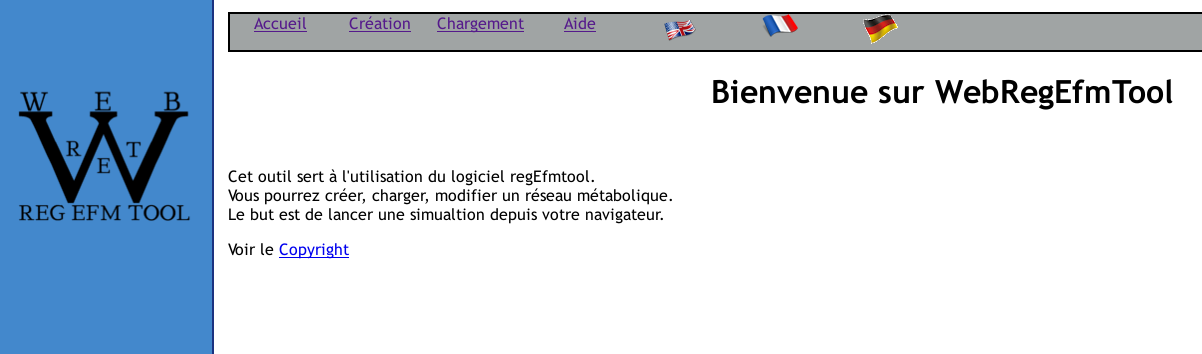
\includegraphics[width=0.90\textwidth]{../Images/Rapport/pageAccueil.png}  
		 \end{minipage}}
		\caption{Page d'accueil}
  		\label{main}
  	\end{center}	
\end{figure}

Lorsqu'un utilisateur arrive sur le site, une page d'accueil s'affiche (Figure \ref{main}). Elle contient des informations relatives à l'utilisation du programme (à quoi il sert, que peut-on y faire ...). A partir de là, deux choix s'offrent à lui:
\begin{itemize}
\item Soit il créé un nouveau réseau, en cliquant sur \emph{Création} dans le menu situé en haut de page,
\item Soit il charge un réseau qu'il a déjà créé en cliquant sur \emph{Chargement}.\\
\end{itemize}

Chaque page du site se présente de la m\^eme façon: un menu en haut de la page et le logo du site Web dans un bandeau situé sur la gauche.\\
Le menu contient quatre onglets:
\begin{itemize}
\item \emph{Accueil} qui permet de retourner sur la page d'accueil du site Web,
\item \emph{Création} qui permet de créer un nouveau réseau métabolique,
\item \emph{Chargement} qui permet de charger un réseau pré-existant,
\item \emph{Aide} qui permet de consulter une aide à l'utilisation du site.
\end{itemize}
On trouve aussi dans le menu, trois drapeaux qui permettent de changer la langue du site Web. Les trois langues proposées sont: l'anglais, le français et l'allemand. Par défaut le site est en français.

%~~~~~~~~~~~~~~~~~~~~~~~~~~~~~
\section{Création d'un nouveau réseau}
%~~~~~~~~~~~~~~~~~~~~~~~~~~~~~

Si l'utilisateur choisi de créer un nouveau réseau, il arrive sur une page qui va lui permettre d'ajouter de nouvelles réactions à celui-ci. \\

Une première partie permet d'initialiser les fichiers (Figure \ref{creation1}) dans le cas où l'utilisateur aurait déjà créé un réseau précédemment.\\

\begin{figure}[!ht]
	\begin{center}
		\fbox{
   		 \begin{minipage}[c]{0.9\textwidth}
  			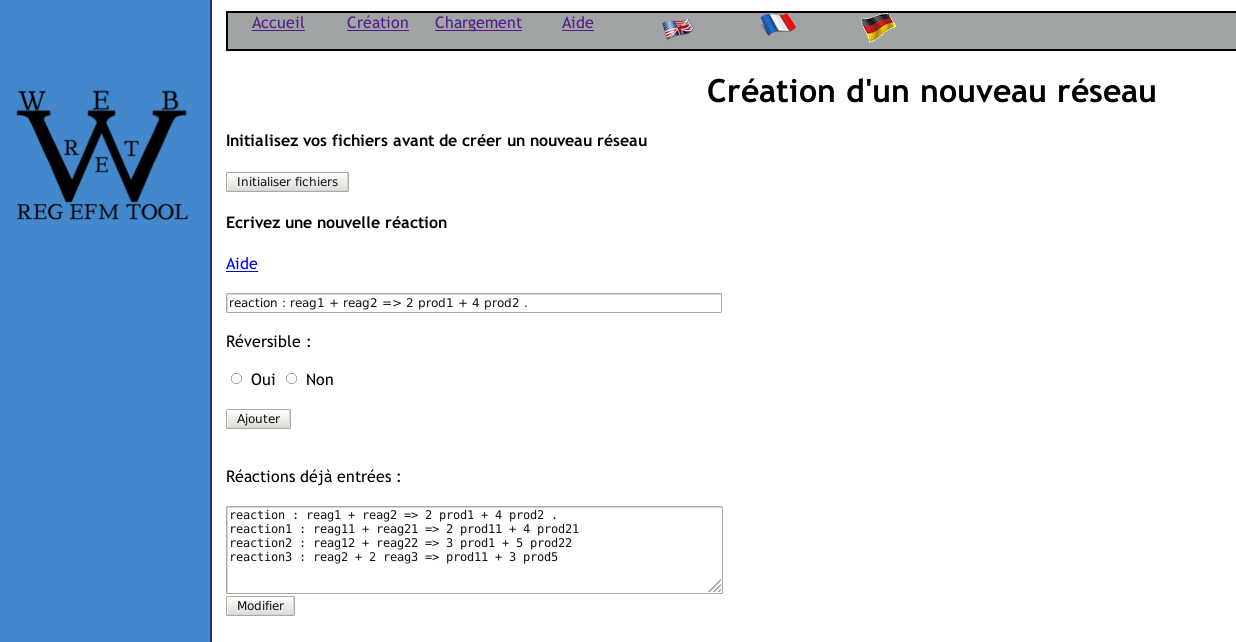
\includegraphics[width=0.90\textwidth]{../Images/Rapport/creation1.png}  
		 \end{minipage}}
		\caption{Page de création d'un nouveau réseau}
  		\label{creation1}
  	\end{center}	
\end{figure}

Une seconde partie permet de créer une nouvelle réaction. Celle-ci doit être de la forme $reaction : reag1 + reag2 => 2 prod1 + 4 prod2$. \\
L'utilisateur doit également préciser si la réaction est réversible ou non. Ensuite il clique sur le bouton \emph{Ajouter}, la réaction est alors ajoutée au réseau et apparaît dans la zone de texte située en-dessous. Dans cette zone de texte, l'utilisateur a la possibilité de modifier les réactions déjà créées (mais ne peut pas en ajouter ou en supprimer car les règles de réversibilités ne seraient alors pas respectées pour l'écriture d'un fichier au format \emph{.dat}). Il valide ensuite les modifications apportées en cliquant sur le bouton \emph{Modifier}.\\

\begin{figure}[!ht]
	\begin{center}
		\fbox{
   		 \begin{minipage}[c]{0.9\textwidth}
  			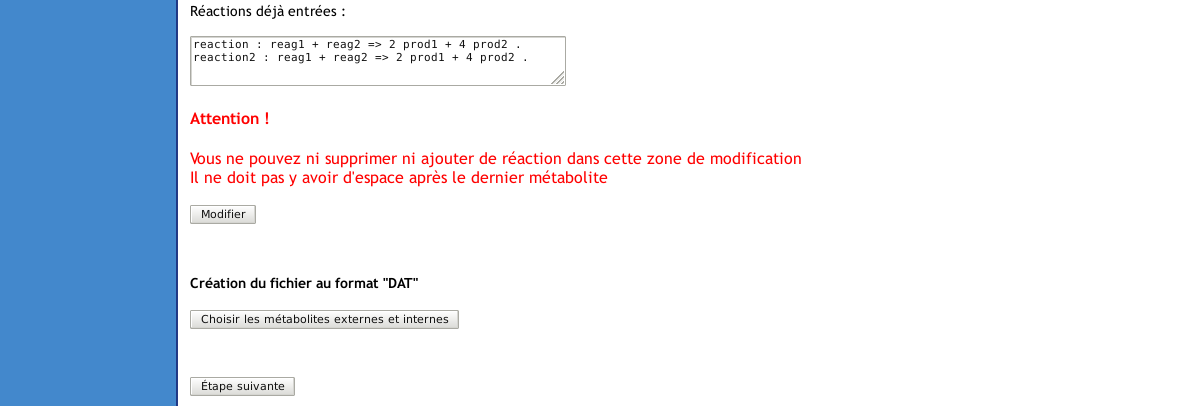
\includegraphics[width=0.90\textwidth]{../Images/Rapport/creation2.png}  
		 \end{minipage}}
		\caption{Suite de la page de création}
  		\label{creation2}
  	\end{center}	
\end{figure}

Enfin, l'utilisateur peut aussi générer un fichier au format \emph{.dat} (Figure \ref{creation2}) qui pourra être utilisé dans METATOOL par exemple.\\

\begin{figure}[!ht]
	\begin{center}
		\fbox{
   		 \begin{minipage}[c]{0.9\textwidth}
  			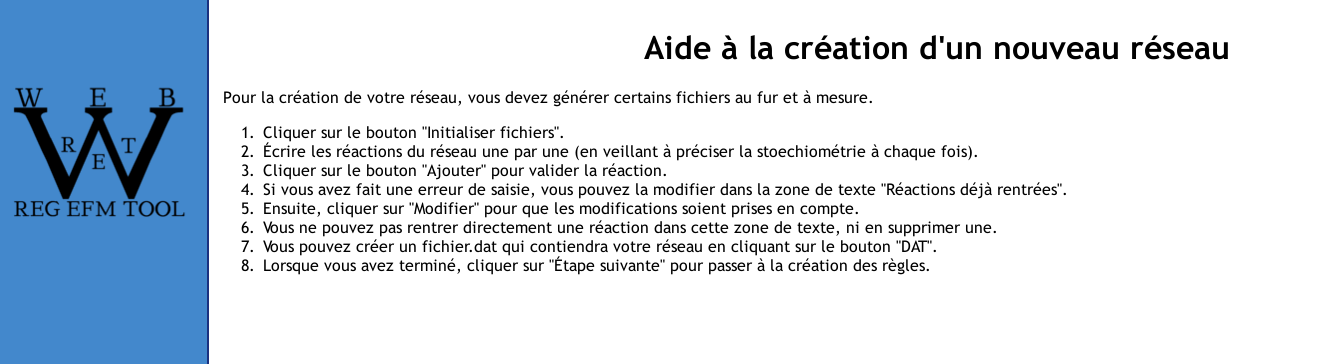
\includegraphics[width=0.90\textwidth]{../Images/Rapport/helpCreation.png}  
		 \end{minipage}}
		\caption{Page d'aide à la création d'un nouveau réseau}
  		\label{helpCreation}
  	\end{center}	
\end{figure}

Si l'utilisateur ne sait pas comment faire, il lui suffit de cliquer sur \textit{Aide} et une nouvelle fen\^etre de navigation (Figure \ref{helCreation}) appara\^itra afin de la guider. Cette page est automatiquement traduite dans la langue de la page courante. 

Quand l'utilisateur a fini de créer toutes les réactions qui composent son réseau, il clique sur le bouton \emph{\'Etape suivante} et arrive alors sur la page de création des règles des gènes.

%~~~~~~~~~~~~~~~~~~~~~~~~~~~~~
\section{Règles des gènes}
%~~~~~~~~~~~~~~~~~~~~~~~~~~~~~

Ces règles sont utilisées pour éliminer les modes élémentaires non possibles dans un réseau métabolique réel.\\

Une réaction R peut \^etre 1-active (R=1), 0-active (R=0) ou encore full-active (R=f).\\
La création des règles est régie selon certains principes:
\begin{itemize}
\item La réaction de sortie ne peut jamais être une réaction d'entrée. \\On ne peut pas écrire: R3 = ( ! ( ( ! 0R3) $|$  1R1) )
\item Une réaction peut être utilisée plusieurs fois comme réaction d'entrée. \\Ex: R11 = ( ( ! ( ( ! 0R3) $|$ 1R5) ) \& 1R3)
\item Le préfixe d'une réaction n'est valable que pour une opération.\\ Ainsi dans la règle R11 = ( ( ! ( ( ! 0R3) $|$ 1R5) ) \& 1R3), la réaction R3 est 0-active dans l'opération OR et 1-active dans l'opération AND.
\item Chaque réaction doit être entourée d'exactement une paire de parenthèses. \\R3 = ( ! 0R1 ) est correcte, mais R3 = ( ( ! 0R1) ) et R3 = ! 0R1 sont incorrectes
\item Il n'existe pas d'opération permettant de représenter la relation R2 = R1, elle sera représentée de la façon suivante: R2 = (fR1 $|$ fR1).\\
\end{itemize}

\begin{figure}[!ht]
	\begin{center}
		\fbox{
   		 \begin{minipage}[c]{0.9\textwidth}
  			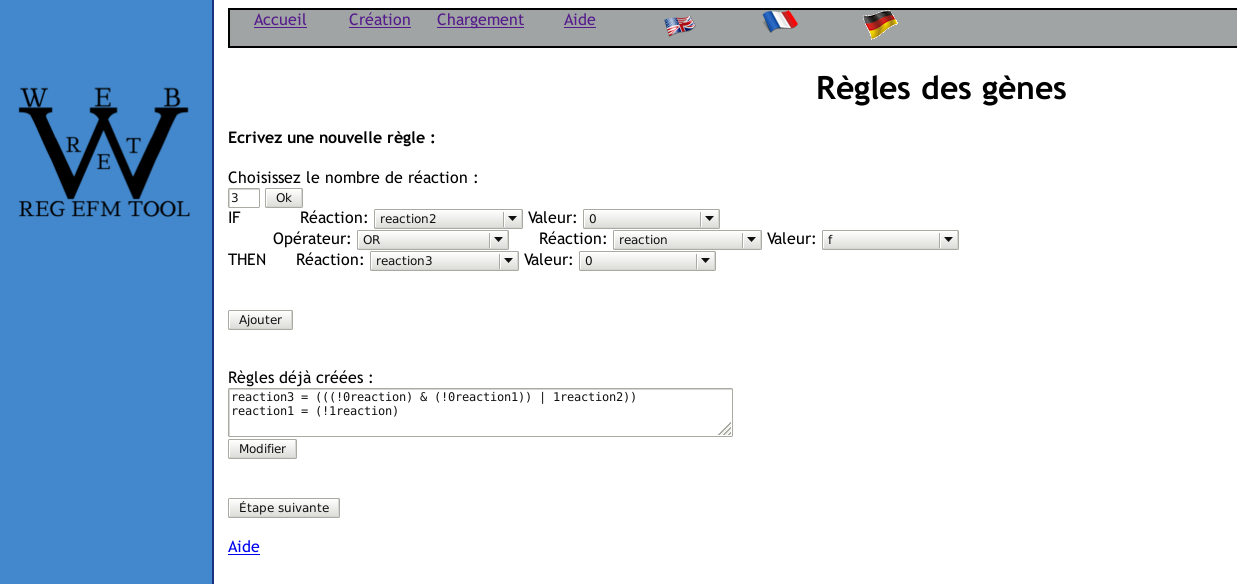
\includegraphics[width=0.90\textwidth]{../Images/Rapport/generules.png}  
		 \end{minipage}}
		\caption{Page de création des règles des gènes}
  		\label{generules}
  	\end{center}	
\end{figure}

Tout d'abord, l'utilisateur choisi le nombre de réactions qui composent la règle qu'il veut créer.
Une fois ce choix effectué, il clique sur le bouton \emph{Ok}. S'affichent alors de deux ou trois menus déroulant par réaction. Quand il y en a trois (Figure \ref{generules}), le premier permet de choisir l'opérateur, le second la réaction et le dernier sa valeur (0, 1 ou f). Quand il y en a deux, ils correspondent à la réaction et à sa valeur. L'utilisateur doit entrer un nombre de réactions au moins égal à deux.\\

L'utilisateur ne peut sélectionner le nom d'une réaction que lorsqu'il a choisi la précédente. Ceci permet de ne proposer que les réactions non sélectionnées précédemment pour le choix de la  réaction de sortie (principe utilisé dans la documentation de \emph{regEfmtool}).\\

Enfin, quand l'utilisateur a sélectionné toutes les réactions ainsi que leur valeur, il clique sur le bouton \emph{Ajouter}. La règle est alors écrite dans le fichier \emph{generules.grfile} si l'utilisateur a bien rempli tous les champs. Celle-ci apparaît alors dans la zone de texte située en-dessous. Dans cette zone, l'utilisateur a la possibilité de modifier, ajouter ou supprimer une règle déjà écrite, mais également d'en écrire de nouvelles manuellement. Lorsqu'il a fini ses modifications, il clique sur le bouton \emph{Modifier}, le fichier \emph{generules.grfile} est alors modifié en conséquence.\\

\begin{figure}[!ht]
	\begin{center}
		\fbox{
   		 \begin{minipage}[c]{0.9\textwidth}
  			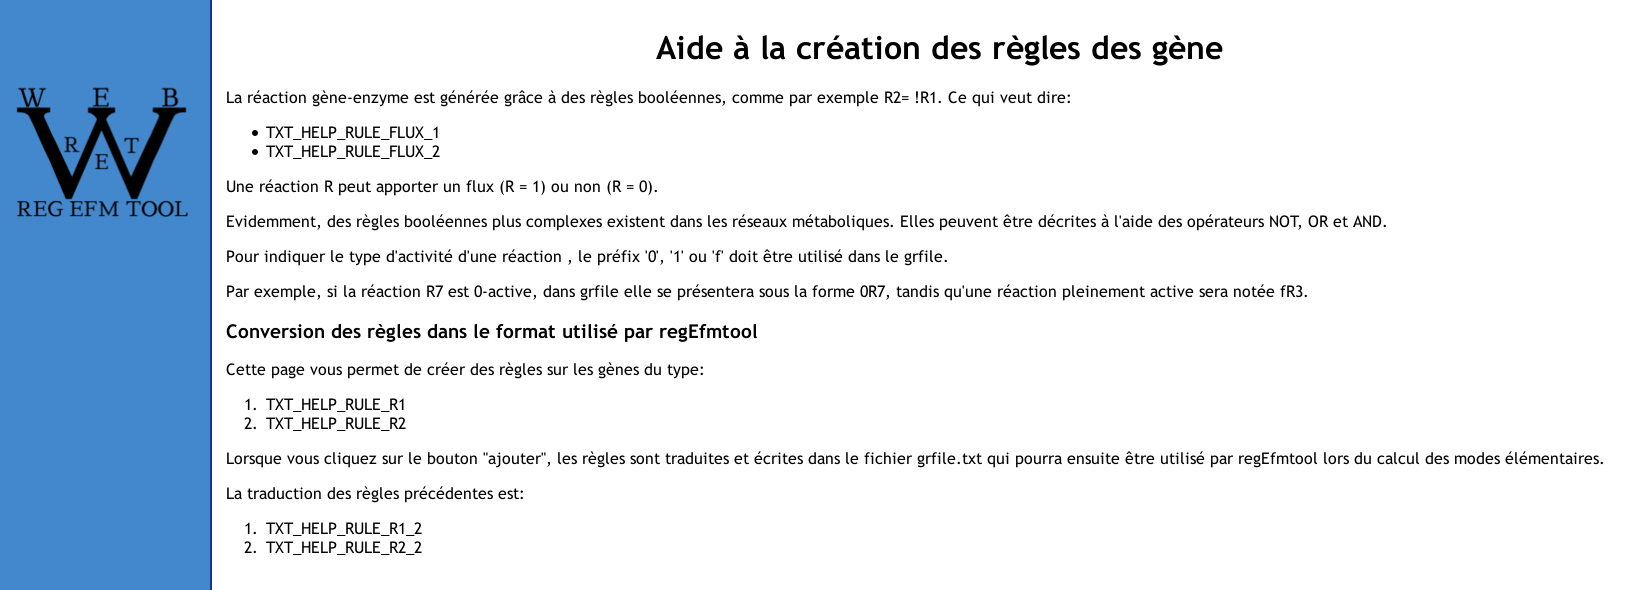
\includegraphics[width=0.90\textwidth]{../Images/Rapport/helpGenerules.png}  
		 \end{minipage}}
		\caption{Page d'aide à la création des règles des gènes}
  		\label{helpGenerules}
  	\end{center}	
\end{figure}

Si l'utilisateur ne sait pas comment faire, il lui suffit de cliquer sur \textit{Aide} comme précédemment et une nouvelle fen\^etre de navigation (Figure \ref{helpGenerules}) appara\^itra afin de la guider. Cette page est également automatiquement traduite dans la langue de la page courante. 

Une fois les règles entrées, l'utilisateur peut passer à l'étape suivante en cliquant sur le bouton correspondant. Il arrive alors sur la page de sélection des options nécessaires au lancement de la commande regEfmtool.

%~~~~~~~~~~~~~~~~~~~~~~~~~~~~~
\section{Choix des options de lancement}
%~~~~~~~~~~~~~~~~~~~~~~~~~~~~~

Comme nous l'avons dit précédemment, regEfmtool se lance gr\^ace à une ligne de commande. Cette page d'options (Figure \ref{options}) permet donc à l'utilisateur de sélectionner les paramètres de calcul qu'il souhaite, par la biais de boutons à cocher. Certaines options sont pré-cochées, se sont les options de base nécessaires au bon déroulement des calculs du logiciel. Cela permet à un utilisateur non expérimenté de lancer ses calculs avec le réseau qu'il vient de créer. Un utilisateur plus averti pourra modifier ces options à sa guise afin d'avoir un niveau de complexité d'exécution des calculs supérieur.\\

\begin{figure}[!ht]
	\begin{center}
		\fbox{
   		 \begin{minipage}[c]{0.9\textwidth}
  			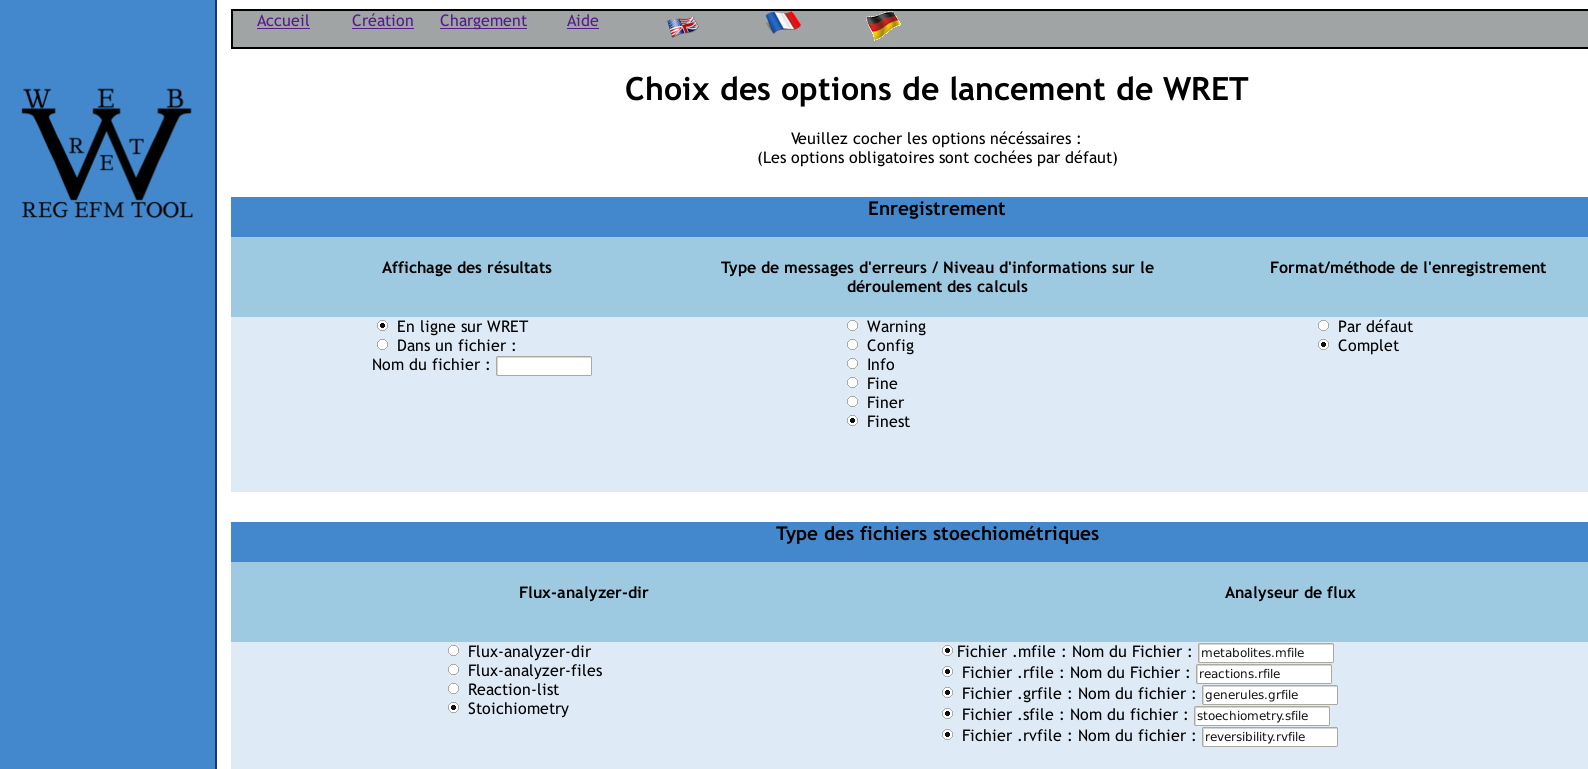
\includegraphics[width=0.90\textwidth]{../Images/Rapport/options.png}  
		 \end{minipage}}
		\caption{Partie de la page de choix des options de lancement}
  		\label{options}
  	\end{center}	
\end{figure}

Les options sont regroupées par catégories (en fonction de ce qui était précisé dans le fichier \textit{metabolic-efm.xml} de regEfmtool):

\paragraph*{Enregistrement} Cette catégorie contient trois sous catégories précisant le type d'affichage des résultats, le niveau d'informations sur le déroulement des calculs et le format d'enregistrement. Par défaut, l'affichage se fera en ligne sur le site et le type de message d'information est le plus complet possible. 

\paragraph*{Types de fichiers stœchiométriques} Cette catégorie possède deux sous catégories précisant le type de parsage en entrée et l'analyseur de flux. Cette dernière permet de définir les types de fichiers d'entrée que regEfmtool utilisera. Ces fichiers étant lors des étapes précédentes, leurs noms sont déjà pré-rentrés dans les cases correspondantes.

\paragraph*{Compression et paramètres de sortie} Ces deux catégories contiennent chacune une seule sous catégorie, servant respectivement à définir le niveau de compression (et également l'utilisation de la récursivité dans les calculs) et le type de fichier désiré en paramètre de sortie. L'option "text-doubles" est cochée par défaut, avec le nom du fichier qui contiendra les modes élémentaires calculés. Nous avons appelé ce fichier \textit{results.txt}. 

\paragraph*{Paramètres d'Efmtool} Cette dernière catégorie contient sept sous catégories: le "\textit{rowordering}" (ou la ligne de commande à utiliser), la méthode d'adjacence, le nombre maxiamal de "\textit{threads}" (prédéfini à 2 suivant les exemples de regEfmtool), l'arithmétique des nombres, le type de normalisation pour la sortie (prédéfinie à "aucune"), la précision fractionnaire et l'activation ou non d'un auto-test après chaque itération. \\

Une fois que l'utilisateur a coché toutes les options qu'il souhaite, il lui suffit de cliquer sur le bouton \emph{Lancement} afin de générer la commande et lancer regEfmtool. Ensuite, une page d'affichage des résultats s'affiche. 

%~~~~~~~~~~~~~~~~~~~~~~~~~~~~~
\section{Chargement d'un réseau pré-existant}
%~~~~~~~~~~~~~~~~~~~~~~~~~~~~~

\subsection{Choix des paramètres}
Cette page accessible depuis le menu général permet à un utilisateur de charger un réseau préexistant depuis son disque dur (Figure \ref{chargement1}). Il pourra également générer la ligne de commandes nécessaire au lancement de regEfmtool. Cette page est basée sur le modèle de la page du choix des options après création, à un détail près : dans la catégorie du type des fichiers stœchiométriques, il n'y a plus la sous-catégorie des fichiers d'analyseur de flux. Le reste fonctionne de la m\^eme façon que précédemment. \\

\begin{figure}[!ht]
	\begin{center}
		\fbox{
   		 \begin{minipage}[c]{0.9\textwidth}
  			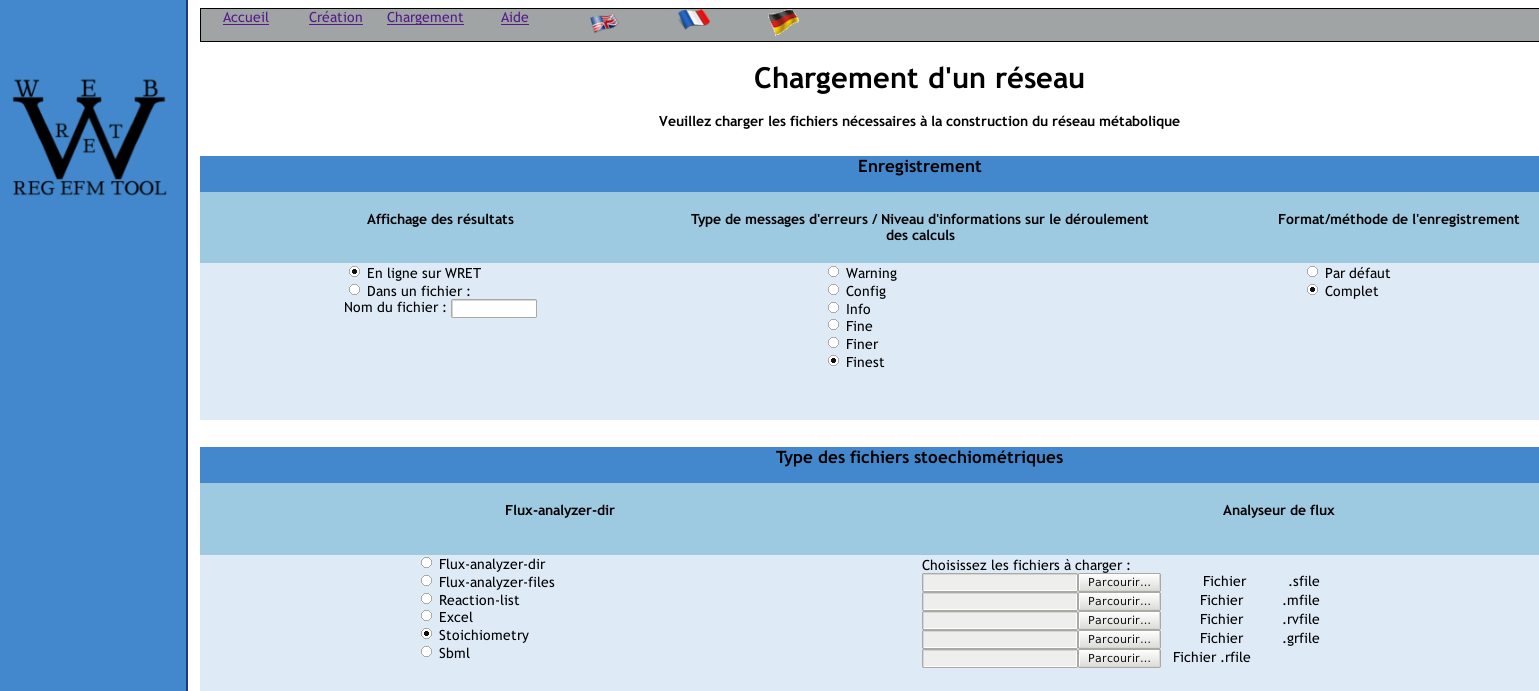
\includegraphics[width=0.90\textwidth]{../Images/Rapport/chargement.png}  
		 \end{minipage}}
		\caption{Partie de la page de chargement d'un réseau préexistant}
  		\label{chargement1}
  	\end{center}	
\end{figure}

L'utilisateur n'aura plus qu'à cliquer sur \textit{Lancement} pour lancer la création de la ligne de commande. Cependant, la ligne de commande générée n'est pas la m\^eme qu'après l'étape de création: elle est incomplète. Tous les paramètres concernant les fichiers d'entrée seront récupérés lors du clic sur le bouton \textit{Étape suivante}. 

\subsection{Chargement des fichiers}
Cette page permet à l'utilisateur de sélectionner les fichiers à charger depuis son disque dur. Il y a un ordre précis du type des fichiers à charger (indiqué à l'utilisateur). 

%\begin{figure}[!ht]
%	\begin{center}
%		\fbox{
%   		 \begin{minipage}[c]{0.9\textwidth}
%  			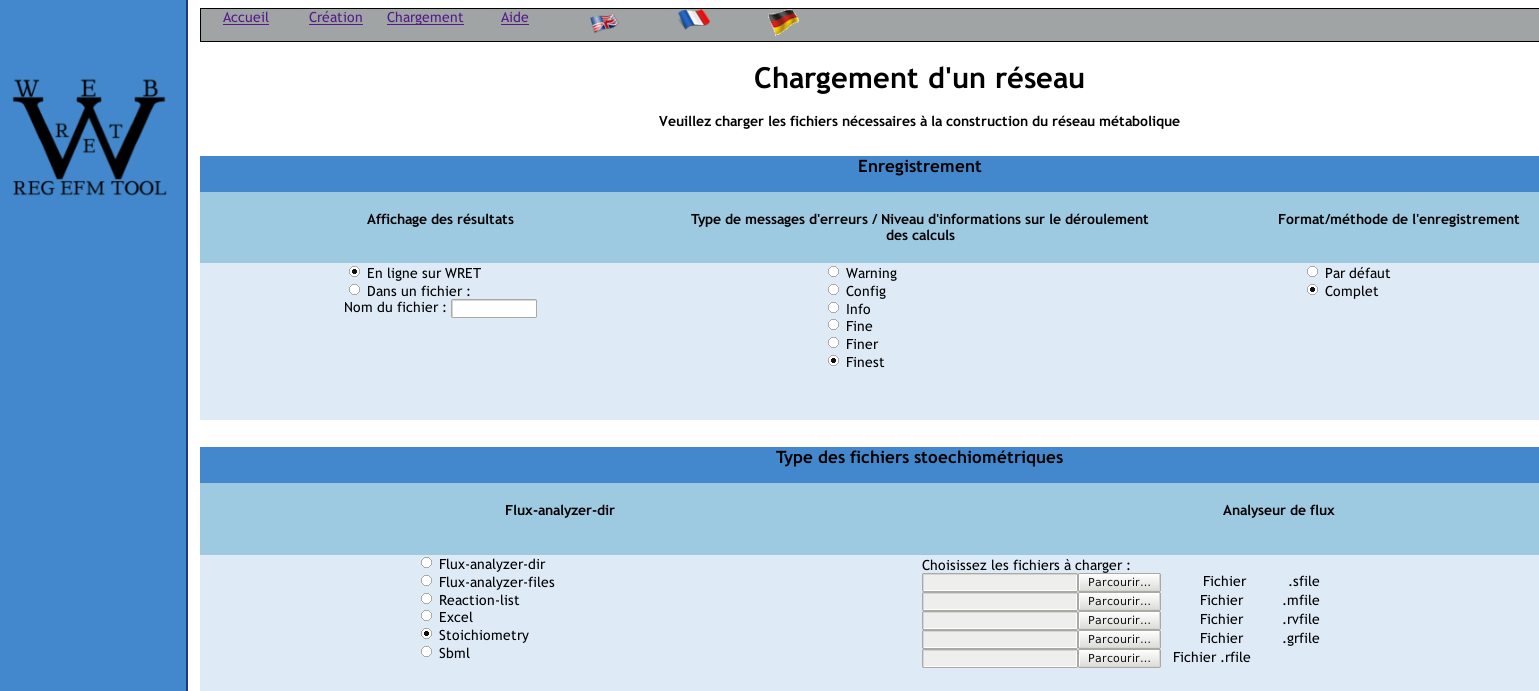
\includegraphics[width=0.90\textwidth]{../Images/Rapport/chargement.png}  
%		 \end{minipage}}
%		\caption{Partie de la page de chargement d'un réseau préexistant}
%  		\label{chargement2}
%  	\end{center}	
%\end{figure}

Une fois les fichiers sélectionnés, il suffit de cliquer sur \textit{Submit} pour effectuer le chargement. Ensuite, l'utilisateur devra cliquer sur "\textit{Résultats}" pour être dirigé vers la page d'affichage des résultats.  

%~~~~~~~~~~~~~~~~~~~~~~~~~~~~~
\section{Affichage des résultats}
%~~~~~~~~~~~~~~~~~~~~~~~~~~~~~














 

%%%%%%%%%%%%%%%%%%%%%%%%%%%%%%
\chapter{Réalisation}
%%%%%%%%%%%%%%%%%%%%%%%%%%%%%%

Nous allons intégrer des digrammes d'organisation des pages Web le long de notre explication afin d'avoir un support visuel. La légende est représentée dans la Figure \ref{DiagLegende}.

\begin{figure}[!ht]
	\begin{center}
		\fbox{
   		 \begin{minipage}[c]{0.4\textwidth}
  			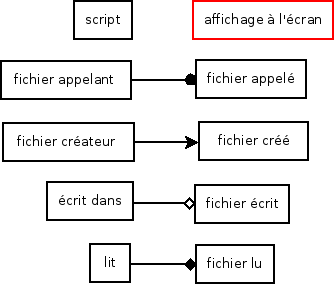
\includegraphics[width=0.90\textwidth]{../WRET/Diagramme/legende.png}  
		 \end{minipage}}
		\caption{Légende de nos diagrammes d'organisation}
  		\label{DiagLegende}
  	\end{center}	
\end{figure}

%~~~~~~~~~~~~~~~~~~~~~~~~~~~~~
\section{Ergonomie de l'interface}
%~~~~~~~~~~~~~~~~~~~~~~~~~~~~~

\subsection{Mise en page}
Nous avons utilisé le CSS afin de régler la mise en page de notre interface. Nous avons intégré une bande verticale sur la gauche du site, contenant un logo de notre création. Nous avons dû adapter la zone d'affichage en fonction de cette bande, mais également faire attention à ce que l'affichage soit ajusté à la taille de l'écran de l'utilisateur. Ce dernier critère était très important, notamment pour l'affichage du menu des onglets en haut des pages, mais aussi pour celui des pages de choix d'options de lancement. 

\paragraph*{Exemple de la page du choix des options}
Cette page est composée d'un emboîtement de plusieurs sections, grâce à la balise HTML \texttt{<div>}, qui est une sorte de conteneur. Comme nous l'avons précisé précédemment, nous avons séparé les options en plusieurs catégories et sous-catégories, distinguées par une combinaison de dégradé de bleus. 

\begin{figure}[!ht]
	\begin{center}
		\fbox{
   		 %\begin{minipage}[c]{1.1\textwidth}
  			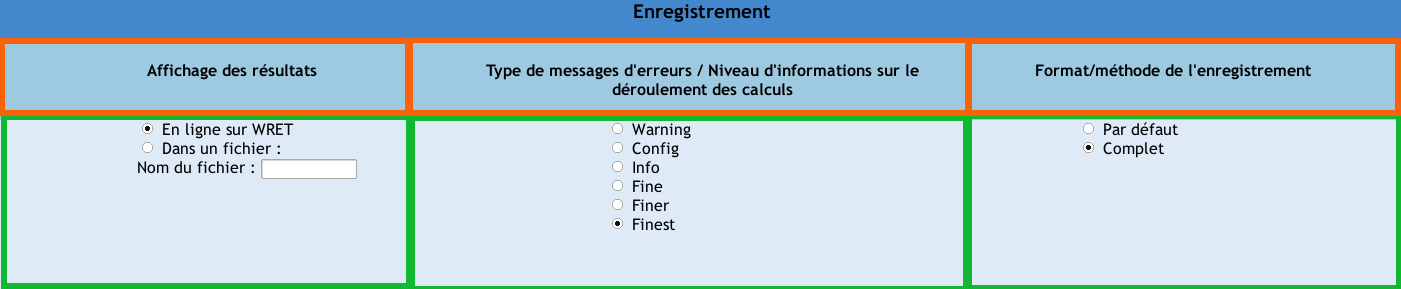
\includegraphics[width=1.0\textwidth]{../Images/Rapport/options-2.png}  
		 %\end{minipage}}
		 }
		\caption{Exemple d'organisation d'une catégorie}
  		\label{categorieCSS}
  	\end{center}	
\end{figure}

Nous avons pris l'exemple des paramètres d'enregistrement des fichiers avec trois sous-catégories, contenu dans une \textit{division}. 
\begin{itemize}
\item L'intitulé de la catégorie générale (\textit{Enregistrement}) est en bleu foncé (le même que celui de la bande verticale) et représente une sorte de \textit{sous-division}. 
\item Les titres des trois sous catégories (\textit{Affichage des résultats}, \textit{Type de messages d'erreurs} et \textit{Méthode d'enregistrement}) sont en bleu clair et représentent également une \textit{sous division}. Cette dernière est aussi divisée en trois sortes de \textit{sous-sous-division} (en orange).
\item Les contenus correspondants aux trois sous catégories sont également divisés en trois \textit{sous-sous-division} (en vert).
\end{itemize} 

Il a fallu ajuster la taille de ces sous catégories de manière relative à la taille de l'écran. Voici un exemple du code CSS correspondant:\\

\begin{DDbox}{\linewidth}
\begin{lstlisting}
div#part {
 	text-align: center;
	width:100%;
	height: 40px;
	background-color:#4388CC;
	margin-top: 30px;
	margin-bottom: 0px;
	padding: 0px;}
div#subPart {
	margin-bottom: 0px;
	margin-top: 0px;
	width:100%;
	height: 80px;
	background-color:#9ECAE1;
	padding: 0px;}
div#subPart3-2 {
	float:left;
	width:33.3%;
	height:60px;
	background-color:#9ECAE1;
	text-align: center;}
div#buttons {
	width:100%;
	height:175px;
	background-color:#DEEBF7;
	clear:both;}
div#buttons3-2 {
	float:left;
	width:33.3%;
	height:140px;
	background-color:#DEEBF7;
	text-align: justify;
	margin-right: -10%;
	margin-left: 10%;}
\end{lstlisting}
\end{DDbox}

La \texttt{div\#part} est utilisée pour le titre de la catégorie. Sa hauteur est fixe mais sa largeur s'adapte à celle de l'écran. La \texttt{div\#subPart} sert de conteneur à \texttt{div\#subPart3-1}, \texttt{div\#subPart3-2} et \texttt{div\#subPart3-3}  qui sont en vert (ici, seul le code relatif à \texttt{div\#subPart3-2} est montré pour des raisons d'économie de place car les 3 sont très semblables). De la même manière, \texttt{div\#buttons} contient \texttt{div\#buttons3-1} \texttt{div\#buttons3-2} \texttt{div\#buttons3-3} qui sont en orange. 

\subsection{Langues}
Dans un soucis de convivialité, notre interface est développée de manière à pouvoir être traduite aisément et propose trois langues possibles dans sa version actuelle (français par défaut, anglais et allemand). Pour changer la langue, l'utilisateur n'a qu'à cliquer sur le drapeau correspondant dans le menu en haut de page. Cela fera appel au script \emph{choosen\_languages.php} (Figure \ref{DiagLangues}), qui lui-même fait appel à \emph{de\_lang.php} pour l'allemand, \emph{en\_lang.php} pour l'anglais et \emph{fr\_lang.php} pour le français, en fonction du drapeau sélectionné. \\
Le fichier \emph{choosen\_languages.php} verifie  soit dans la barre d'adresse soit dans les variables de session php la langue selectionnée par l'utilisateur.\\

\begin{DDbox}{\linewidth}
\begin{lstlisting}
session_start();
	if (isset ($_SESSION['lang']) && !isset($_GET['lang'])){
		$lang=$_SESSION['lang'];
	}
	else if (isset($_GET['lang'])){
		$lang=$_GET['lang'];
		$_SESSION['lang']=$lang;
	}
\end{lstlisting}
\end{DDbox}\\

\begin{figure}[!ht]
	\begin{center}
		\fbox{
   		 \begin{minipage}[c]{0.8\textwidth}
  			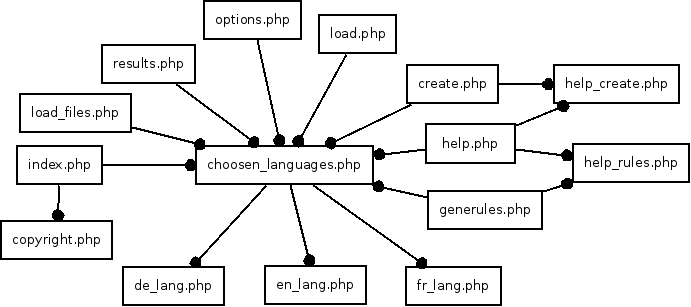
\includegraphics[width=0.90\textwidth]{../WRET/Diagramme/langues.png}  
		 \end{minipage}}
		\caption{Diagramme d'organisation pour le changement de langue}
  		\label{DiagLangues}
  	\end{center}	
\end{figure}

Pour ce faire, nous n'avons pas mis de texte dans les pages affichant à l'écran. Nous l'avons remplacé par des variables, qui afficheront le texte qu'elles contiennent dans la langue désirée. Par exemple, le titre de la page d'accueil "Bienvenue sur WebRegEfmTool" est appelé par \texttt{<?php echo TXT\_HOMEPAGE\_TITLE; ?>} et est contenu dans le fichier \emph{fr\_lang.php} de la manière suivante :
\texttt{define('TXT\_HOMEPAGE\_TITLE', 'Bienvenue sur WebRegEfmTool');}. De ce fait, un nouveau fichier du type \emph{XX\_lang.php} pourrait être créé afin d'intégrer une nouvelle langue. Bien sûr, il faudrait ajouter les appels à ce fichier dans toutes les pages affichant à l'écran par la suite. 

%~~~~~~~~~~~~~~~~~~~~~~~~~~~~~
\section{Création d'un nouveau réseaux}
%~~~~~~~~~~~~~~~~~~~~~~~~~~~~~

\subsection{Initialisation des fichiers}
La création d'un nouveau réseaux dans WRET se fait via la page \emph{create.php}.
A partir de cette page, l'utilisateur doit dans un premier temps appuyer sur le bouton \emph{Initialiser les fichiers} (Figure \ref{boutonInit}) s'il désire initialiser ses fichiers.

\begin{figure}[!ht]
    \begin{center}
        \fbox{
            \begin{minipage}[c]{0.5\textwidth}
              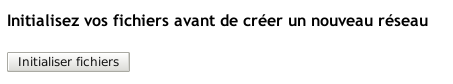
\includegraphics[width=0.90\textwidth]{../Images/Rapport/creation1-1.png} 
         \end{minipage}}
        \caption{Bouton d'initialisation des fichiers}
          \label{boutonInit}
      \end{center}   
\end{figure}

Ce bouton appelle le fichier \emph{initfiles.php} qui va créer les 11 fichiers nécessaires à la mise en place d'un nouveau réseau.\\
Dans ces fichiers, nous trouvons des fichiers qui seront utilisés dans le lancement de \emph{regEfmtool} (rfile, mfile, rvfile, sfile) et également des fichiers temporaires (\emph{irrevTemp}, \emph{revTemp}, \emph{reactionTemp.txt}, \emph{reactionTemp2.txt}, \emph{matrice.txt} ou encore \emph{matrice2.txt} ainsi que la base du fichier au format \emph{DAT}).\\
Tous ces fichiers sont donc créés et donnent les droits d'édition, de lecture et d'exécution à tous les utilisateurs pour chacun d'entre eux, afin de pouvoir être modifiés sur le serveur.

\subsection{Réactions et réversibilité}
Sous la touche \emph{Initialiser les fichiers} de la page \emph{create.php}, une fenêtre de texte permet de rentrer les réactions du réseau métabolique une à une ainsi que la réversibilité de la réaction (Figure \ref{boutonAjout}).

\begin{figure}[!ht]
    \begin{center}
        \fbox{
            \begin{minipage}[c]{0.7\textwidth}
              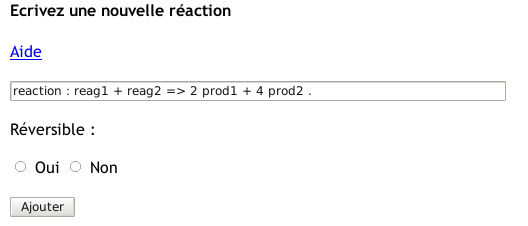
\includegraphics[width=0.90\textwidth]{../Images/Rapport/creation1-2.png} 
         \end{minipage}}
        \caption{Bouton d'ajout d'une réaction}
          \label{boutonAjout}
      \end{center}   
\end{figure}

Si l'utilisateur oublie de cocher la réversibilité de la réaction et clique sur \emph{Ajouter}, un message d'erreur s'affichera et empêchera le passage à l'étape suivante. Les réactions doivent être enregistrées par l'utilisateur en respectant la syntaxe des fichier au format \emph{DAT}. Ces informations vont alors être envoyées au fichier \emph{createFiles.php}, via le bouton \emph{Ajouter}.\\
Ce fichier redirige vers différentes pages, dans l'ordre : \emph{reac.php}, \emph{parser\_enzyme.php},
\\ \emph{parser\_reversibility.php}, \emph{parser\_metabolite.php}, \emph{parser\_stoechiometry.php}.
La première page \emph{reac.php} va permettre d'écrire dans un fichier temporaire (\emph{reactionTemp.txt}) les réactions, et également, de sauvegarder la réversibilité de la réaction (0 pour non réversible, et 1 pour réversible).\\
L'ordre est ainsi conservé entre les réactions et leur réversibilité.

\subsection{Nom de réactions : enzymes}
Une fois les données de réactions et de réversibilité enregistrées, la page \emph{parser\_enzymes.php} est appelée. Elle va parser le fichier temporaire des réactions (\emph{reactionTemp.txt}) et va extraire le premier élément de la réaction situé avant le ":", qui se trouve être le nom de la réaction (nom de l'enzyme généralement).\\
Ces noms sont enregistrés dans un fichier (\emph{reaction.rfile}) en respectant les espaces et la syntaxe nécessaire à l'utilisation au sein de \emph{regEfmtool}.

\subsection{Métabolites}
Après enregistrement des enzymes, le fichier \emph{parser\_metabolites.php} est appelé. Ce script va parser le fichier temporaire contenant les réactions (\emph{reactionTemp.txt}) et va enregistrer chacun des métabolites dans un fichier (\emph{meatbolites.mfile}). Au cours de ce parsage, seuls les éléments situés après le nom de l'enzyme seront pris en compte. Les noms présents plusieurs fois dans le fichier de réactions sont enregistrés une seule fois dans le fichier \emph{metabolites.mfile}.

\subsection{Stœchiométrie}
Enfin après génération des fichiers: \emph{rvfile}, \emph{mfile}, \emph{sfile}, \emph{rfile}, le script \emph{parser\_stoechiometry} est appelé. Il va lancer le script \emph{parser\_stoechiometry.py}. Ce dernier permet de générer la matrice de stœchiométrie nécessaire a \emph{regEfmtool}. Pour ce faire, il prend les fichiers \emph{reactionTemp.txt} et \emph{metabolites.mfile} en entrée. Il génère la matrice ligne par ligne (une ligne correspondant à une réaction). \\
Pour chaque ligne du fichier \emph{reactionTemp.txt}, une liste est créée et, pour chaque métabolite de cette réaction, sa stœchiométrie est enregistrée en respectant son ordre dans le fichier contenant les réactifs. Ce script fournit alors en sortie le fichier \emph{stoechiometry.sfile}.

\subsection{Modification du réseaux}
Une fois les fichiers générés, l'utilisateur est redirigé sur la page \emph{create.php}.
Sous la touche \emph{Ajouter} se trouve une zone de texte (Figure \ref{boutonAjout}) où l'utilisateur peut modifier un réseau déjà rentré.

\begin{figure}[!ht]
    \begin{center}
        \fbox{
            \begin{minipage}[c]{0.7\textwidth}
              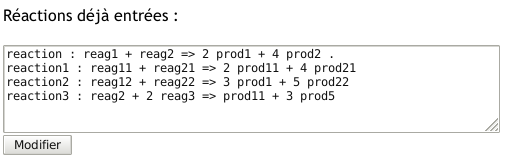
\includegraphics[width=0.90\textwidth]{../Images/Rapport/creation1-3.png} 
         \end{minipage}}
        \caption{Bouton de modification}
          \label{boutonModif}
      \end{center}   
\end{figure}

En effet, cette zone appelle le fichier \emph{reactionTemp.txt} et permet la modification de son contenu (pour corriger une erreur de frappe notamment). Cette zone de texte va appeler la page \emph{modifier.php} lors de l'utilisation du bouton \emph{Modifier}.\\
 Cette page efface le précédant fichier \emph{reactionTemp.txt} et insère le nouveau contenu que l'utilisateur a modifié. \\
 Les fichiers \emph{metabolites.mfile}, \emph{stoechiometry.sfile}, \emph{reactions.rfile}, \emph{reversibility}, sont également générés à nouveau, à chaque modification du fichier \emph{reactionTemp.txt}.
 
\subsection{Création du fichier \emph{DAT}}

En dessous de la zone de texte modifiable, une touche nommée \emph{Choisir les métabolites internes et externes} (Figure \ref{boutonMET_int_EXT}) permet à l'utilisateur de définir dans son réseaux les métabolites internes et externes . Ce bouton va effectuer un parsage du fichier \emph{metabolites.mfile} et afficher dans une colonne à gauche contenant tous les métabolites. Une colonne a droite vide peut être remplie ou vidé via les bouton \emph{Ajouter}, \emph{Supprimer} situés sous les colonnes.
Ces touches d'ajout et de suppression font appelle à des fonctions \emph{javascript}, directement intégrées à la page \emph{create.php}.\\

\begin{figure}[!ht]
    \begin{center}
        \fbox{
            \begin{minipage}[c]{0.5\textwidth}
              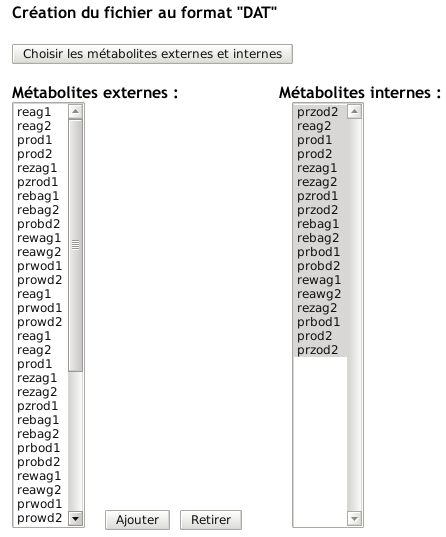
\includegraphics[width=0.9\textwidth]{../Images/Rapport/creation3.png} 
         \end{minipage}}
        \caption{Zone de sélection des métabolites internes et externes}
          \label{boutonMET_int_EXT}
      \end{center}   
\end{figure}

Sous la zone de sélection des métabolites internes et externes, un bouton \emph{DAT} permet de générer un fichier au format \emph{DAT} du réseaux métabolique précédemment rentré. \\

\begin{figure}[!ht]
    \begin{center}
        \fbox{
            \begin{minipage}[c]{0.3\textwidth}
              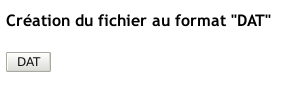
\includegraphics[width=0.90\textwidth]{../Images/Rapport/creation2-1.png} 
         \end{minipage}}
        \caption{Bouton de création du fichier au format \emph{DAT}}
          \label{boutonDAT}
      \end{center}   
\end{figure}

Ce bouton (Figure \ref{boutonDAT}) appelle la page \emph{finish\_files.php} qui va  récupérer les choix de l'utilisateur en ce qui concerne les métabolites internes et externes, et concaténer trois fichiers :
\begin{itemize}
\item \emph{irrevTemp.txt}
\item \emph{revTemp.txt}
\item \emph{reactiontemp2.txt}
\end{itemize}

Le premier fichier contient l'ensemble des enzymes catalysant les réactions irréversibles. Le second contient l'ensemble des enzymes catalysant des réactions réversibles, et enfin le dernier fichier contient l'ensemble des réactions du réseaux. \\
Chacun de ces fichiers contient les balises \emph{-ENZIRREV}, \emph{-ENZREV}, \emph{-CAT}, selon son contenu et respecte la syntaxe propre au format \emph{DAT}.
Les noms des métabolites sont insérés dans le fichier au format \emph{DAT} après une balise \emph{-METINT} ou \emph{-METEXT}, selon leur rôle dans le réseaux défini par l'utilisateur.

Il en résulte en sortie du script \emph{finish\_files.php} un fichier au format \emph{DAT}, de la forme:
\\
\begin{DDbox}{\linewidth}
\begin{lstlisting}
-ENZREV
R9 R12 R13 R14 R15   T1 T2 T5 T7 T12

-ENZIRREV
R6i R7i R8i R10i R11i T6

-METINT
OAA ACoA Cit Akg SucCoA Succ Fum Mal Isocit  Pi  Glu Asp Pyr

-METEXT
Pyr_ext Glu_ext NAD NADH2 FAD FADH2  CoA ADP ATP  H2O CO2 Mal_ext Cit_ext AKG_ext Pi_ext Asp_ext

-CAT

R6i : Pyr + CO2 + ATP = OAA + Pi + ADP .
R7i : Pyr + NAD + CoA = ACoA + NADH2 + CO2 .
R8i : OAA + ACoA + H2O = Cit + CoA .
R9 : Cit = Isocit .
R10i : Isocit + NAD = Akg + NADH2 + CO2 .
R11i : Akg + NAD + CoA = SucCoA + NADH2 + CO2 .
R12 : SucCoA + Pi + ADP = Succ + CoA + ATP .
R13 : Succ + FAD = Fum + FADH2 .
R14 : Fum + H2O = Mal .
R15 : Mal + NAD = OAA + NADH2 .
T1 : Cit + Mal_ext = Mal + Cit_ext .
T2 : AKG_ext + Mal = Mal_ext + Akg .
T5 : Pi_ext = Pi .
T6 : Pyr_ext = Pyr .
T7 : Mal + Pi_ext = Pi + Mal_ext .
T12 : Asp + Glu_ext = Asp_ext + Glu .

\end{lstlisting}
\end{DDbox}

%~~~~~~~~~~~~~~~~~~~~~~~~~~~~~
\section{Règles des gènes}
%~~~~~~~~~~~~~~~~~~~~~~~~~~~~~

\begin{figure}[!ht]
	\begin{center}
		\fbox{
   		 \begin{minipage}[c]{0.7\textwidth}
  			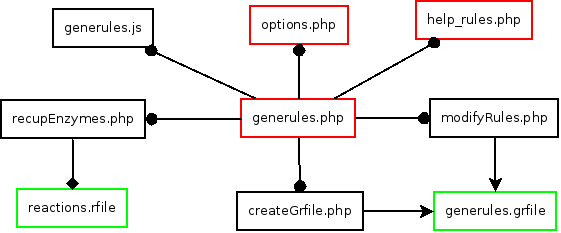
\includegraphics[width=0.90\textwidth]{../WRET/Diagramme/generules.png}  
		 \end{minipage}}
		\caption{Diagramme d'organisation pour le changement de langue}
  		\label{DiagRegles}
  	\end{center}	
\end{figure}

La page permettant la saisie des règles générales est obtenue à l'aide du fichier \emph{generules.php} (Figure \ref{DiagRegles}).\\
L'affichage à l'ouverture de la page n'est composé que d'une zone de texte et d'un bouton \emph{Ok} (Figure \ref{boutonOK}) qui est de type \textit{submit}. 

\begin{figure}[!ht]
	\begin{center}
		\fbox{
   		 \begin{minipage}[c]{0.3\textwidth}
  			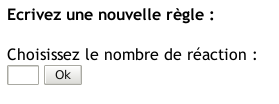
\includegraphics[width=0.90\textwidth]{../Images/Rapport/generules-1.png}  
		 \end{minipage}}
		\caption{Bouton du choix du nombre de réactions pour une règle}
  		\label{boutonOK}
  	\end{center}	
\end{figure}

Au clic, ce bouton fait appel à la fonction \emph{add\_reaction()} qui créée  deux menus déroulants (pour la première et la dernière, Figure \ref{menusDeroulants1}) ou trois menus déroulants (pour les autres, Figure \ref{menusDeroulants2}) par réaction jusqu'à atteindre le nombre de réactions entrées par l'utilisateur. 

\begin{figure}[!ht]
	\begin{center}
		\fbox{
   		 \begin{minipage}[c]{0.7\textwidth}
  			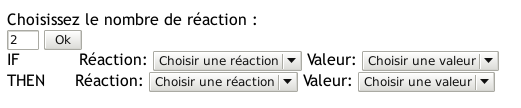
\includegraphics[width=0.90\textwidth]{../Images/Rapport/generules-2.png}  
		 \end{minipage}}
		\caption{Menus déroulant si 2 réactions dans la règle}
  		\label{menusDeroulants1}
  	\end{center}	
\end{figure}

\begin{figure}[!ht]
	\begin{center}
		\fbox{
   		 \begin{minipage}[c]{0.8\textwidth}
  			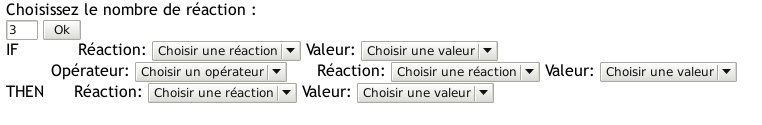
\includegraphics[width=0.90\textwidth]{../Images/Rapport/generules-3.png}  
		 \end{minipage}}
		\caption{Menus déroulant si 3 réactions dans la règle}
  		\label{menusDeroulants2}
  	\end{center}	
\end{figure}

Elle vérifie également que le nombre de réactions entrées par l'utilisateur est au moins égal à 2, sinon elle affiche un message sous la forme d'une alerte à l'utilisateur.\\
Les réactions sont récupérées à partir de \emph{reactions.rfile}.\\

L'utilisateur peut sélectionner plusieurs fois la m\^eme réaction dans sa règle, sauf pour le choix de la dernière (ligne THEN). Cette particularité est gérée par la fonction \texttt{choice(form, val)}. Celle-ci permet de remplir les menus déroulants quand une réaction a été choisie et pour la dernière seules les réactions non sélectionnées précédemment appara\^issent.

Lorsque l'utilisateur a choisi toutes ses réactions, leur opérateur et leur valeur, il clique sur le bouton \emph{Ajouter}. Celui-ci fait appel à la fonction \texttt{validateForm()} qui vérifie que tous les champs ont bien été sélectionnés. Si la fonction retourne VRAI, il fait appel au fichier \emph{createGrfile.php} qui écrit la règle dans le fichier \emph{grfile.txt}.\\
Le fichier \emph{createGrfile.php} écrit dans le fichier \emph{grfile} selon certaines règles. En effet, l'écriture de la règle dépend des valeurs associées aux réactions et des opérateurs choisis.\\

Si la valeur de la réaction qui suit le "THEN" est 0, alors il y aura le symbole "!" au début de la règle (juste après le "="), sauf si la règle ne contient que deux réactions.\\
Si les autres réactions ont pour valeur:
\begin{itemize}
\item 0, alors on écrira (!0reac)
\item 1, alors on écrira (!1reac)
\item f, alors on écrira (!freac)
\end{itemize}
En revanche, si la valeur de la réaction après "THEN" est 1, les autres réactions s'écriront:
\begin{itemize}
\item 0reac si sa valeur est 0
\item 1reac si sa valeur est 1
\item freac si sa valeur est f
\end{itemize}
De plus, si l'opérateur "AND" est sélectionné il sera écrit sous la forme \& dans le fichier, l'opérateur "OR" sera lui écrit $|$. Quand la règle est composée d'au moins trois réactions, des parenthèses sont ajoutées après chaque réaction sauf la première et la dernière. Des parenthèses entourent l'ensemble des réactions situées après le "=".\\

Pour mieux comprendre l'écriture du fichier \emph{generules.grfile}, voici un exemple:\\

Choix de l'utilisateur sur la page Web: \\
\begin{DDbox}{\linewidth}
\begin{lstlisting}
IF reaction: R1 valeur: 1
Operateur: AND reaction: R2 valeur: 0
Operateur: OR reaction: R3 valeur: 0
THEN reaction: R4 valeur: 0
\end{lstlisting}
\end{DDbox}

Règle écrite dans le fichier: \\
\begin{DDbox}{\linewidth}
\begin{lstlisting}
R4 = (!((1R1 \& (!0R2)) $|$ (!0R3))
\end{lstlisting}
\end{DDbox}

%~~~~~~~~~~~~~~~~~~~~~~~~~~~~~
\section{Choix des options de lancement}
%~~~~~~~~~~~~~~~~~~~~~~~~~~~~~

\begin{figure}[!ht]
	\begin{center}
		\fbox{
   		 \begin{minipage}[c]{0.6\textwidth}
  			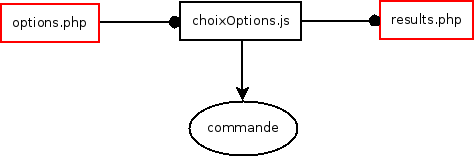
\includegraphics[width=0.90\textwidth]{../WRET/Diagramme/options.png}  
		 \end{minipage}}
		\caption{Diagramme d'organisation pour le choix des options après création}
  		\label{DiagOptions}
  	\end{center}	
\end{figure}

La page permettant la sélection des options de lancement est obtenue à l'aide du fichier \emph{options.php} (Figure \ref{DiagOptions}). Comme nous l'avons dit précédemment, nous avons séparé les options en une série de catégories et sous catégories, le tout contenu dans un formulaire afin de gérer l'interaction avec l'utilisateur. Ce dernier peut sélectionner les options qu'il désire avec une combinaison de \textit{radioboutons} et de zones de texte. Les \textit{radioboutons} d'une même sous-section ont le même attribut \textit{name} afin de ne pouvoir en sélectionner qu'un seul. \\

Prenons comme exemple la première sous catégorie (Figure \ref{affichageResults}) :

\begin{figure}[!ht]
	\begin{center}
		\fbox{
   		 \begin{minipage}[c]{0.3\textwidth}
  			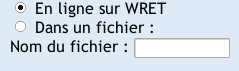
\includegraphics[width=0.90\textwidth]{../Images/Rapport/options-1.png}  
		 \end{minipage}}
		\caption{Sous catégorie d'affichage des résultats dans la catégorie d'enregistrement}
  		\label{affichageResults}
  	\end{center}	
\end{figure}

Voici le code HTML/PHP qui correspond :

\scriptsize
\begin{DDbox}{\linewidth}
\begin{lstlisting}
<input type="radio" name="choix1" value="log console" checked="checked">	<?php echo TXT_OPTIONS_SAVING_3; ?> 
<input type="radio" name="choix1" value="log file"> <?php echo TXT_OPTIONS_SAVING_4; ?> 
<?php echo TXT_OPTIONS_SAVING_5; ?> <input type="text"	 name="log_nomFichier" 	size="10" id="texte1">
\end{lstlisting}
\end{DDbox}

\normalsize

Le premier \textit{radiobouton} est pré-coché avec l'attribut \textit{checked="checked"} afin de guider l'utilisateur. Si cette option ne lui contient pas, il lui suffit de cocher le deuxième \textit{radiobouton} et de remplir la zone de texte associée. \\

Ce sont les attributs \textit{value} de ces boutons qui sont récupérés avec un script JavaScript. Ce dernier, nommé \emph{choixOptions.js}, permet de vérifier quels \textit{radioboutons} sont cochés et récupère ce qu'il a dans l'attribut \textit{value} de ceux-ci quand c'est le cas. Il est appelé lors du clic sur le bouton \textit{Lancement} en bas de la page. De plus, c'est dans ce script qu'est générée la commande qui permettra le lancement de regEfmtool. Elle est contenue dans une variable nommée  \textit{commande}, qui se remplit des paramètres sélectionnés. \\

Exemple du code JavaScript qui permet la récupération des \textit{values} précédentes : \\

\begin{DDbox}{\linewidth}
\begin{lstlisting}
var commande = "java -Xmx1G -jar ../regEfmtool.jar";

  // SAVE
  // Display
  if (formulaire.choix1[0].checked) { 
    valeur1 = " -" + formulaire.choix1[0].value; 
    commande = commande + valeur1;
  }
  else if (formulaire.choix1[1].checked) { 
    var nom1 = document.getElementById('texte1').value;
    valeur1 = " -" + formulaire.choix1[1].value + " " + nom1; 
    commande = commande + valeur1;
  }
\end{lstlisting}
\end{DDbox}

La variable \textit{commande} est une chaîne de caractères qui contient le début de la commande Java. Les paramètres sont ensuite ajoutés au fur et à mesure de la vérification de la sélection des boutons. \\

Cette commande est sauvegardée dans un \textit{cookie} qui sera récupéré à la page d'affichage des résultats pour le lancement de regEfmtool. 

%~~~~~~~~~~~~~~~~~~~~~~~~~~~~~
\section{Chargement d'un réseau pré-existant}
%~~~~~~~~~~~~~~~~~~~~~~~~~~~~~

\begin{figure}[!ht]
	\begin{center}
		\fbox{
   		 \begin{minipage}[c]{0.7\textwidth}
  			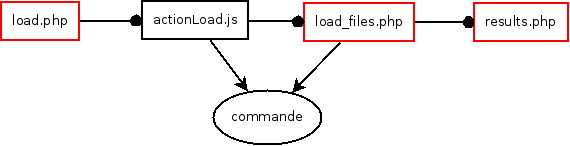
\includegraphics[width=0.90\textwidth]{../WRET/Diagramme/load.png}  
		 \end{minipage}}
		\caption{Diagramme d'organisation pour le chargement des fichiers}
  		\label{DiagLoad}
  	\end{center}	
\end{figure}

Ce sont les pages \emph{load.php} et \emph{load\_files.php} qui permettent le chargement des fichiers contenant un réseau pré-existant (Figure \ref{DiagLoad}) depuis le disque dur de l'utilisateur. Tout d'abord, la page \emph{load.php} permet à ce dernier de choisir les paramètres de la commande de lancement de regEfmtool, de le même façon que pour la page \emph{options.php}. Cependant, la deuxième grande catégorie diffère car le choix des fichiers à charger se fera lors d'une étape ultérieure. Ici, l'utilisateur coche les options qu'il désire et clique sur le bouton \textit{Étape suivante}. Ce bouton fait appel au script JavaScript \emph{actionLoad.js}, qui fonctionne sur le même principe que \emph{choixOptions.js}. \\

Ensuite, l'utilisateur est dirigé vers la page \emph{load\_files.php} (voir figure \ref{choix}) , qui permet à l'utilisateur d'aller "chercher" les fichiers aux formats \textit{sfile}, \textit{mfile}, \textit{rvfile}, \textit{grfile} et \textit{rfile}. Nous copions et renommons ces fichiers dans le dossier courant afin de pouvoir les utiliser dans regEfmtool. Ce processus est faisable grâce au script PHP, dont voici un exemple pour le fichier au format \textit{sfile} :\\

\begin{DDbox}{\linewidth}
\begin{lstlisting}
 move_uploaded_file($_FILES["sfile"]["tmp_name"],$_FILES["sfile"]["name"]);
 shell_exec('mv ' . $_FILES["sfile"]["name"] . ' sfile');
\end{lstlisting}
\end{DDbox}

Ce script est contenu dans l'attribut \textit{value} du bouton de chargement du fichier en question. La ligne de commande est donc complétée et le lancement du logiciel peut commencer. 

\begin{figure}[!ht]
	\begin{center}
		\fbox{
   		 \begin{minipage}[c]{0.9\textwidth}
  			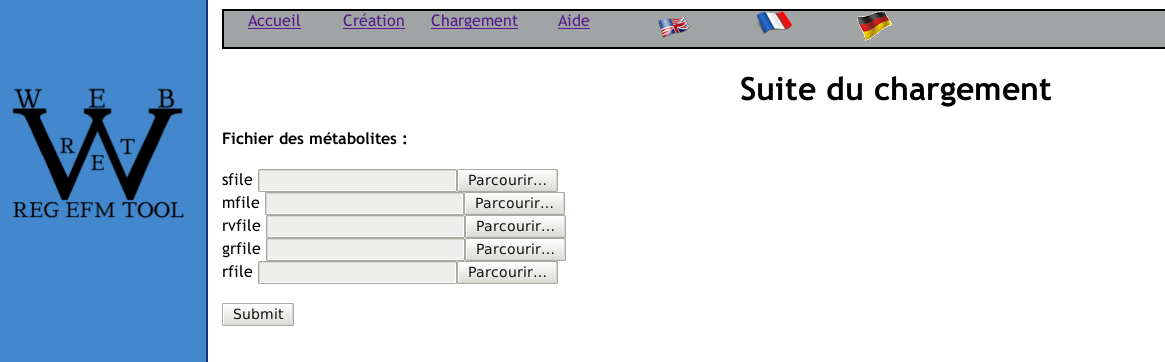
\includegraphics[width=0.90\textwidth]{../Images/Rapport/chargement1.png}  
		 \end{minipage}}
		\caption{Page du choix des fichiers à charger}
  		\label{choix}
  	\end{center}	
\end{figure}

%~~~~~~~~~~~~~~~~~~~~~~~~~~~~~
\section{Affichage des résultats}
%~~~~~~~~~~~~~~~~~~~~~~~~~~~~~

\begin{figure}[!ht]
	\begin{center}
		\fbox{
   		 \begin{minipage}[c]{0.6\textwidth}
  			\includegraphics[width=0.90\textwidth]{../WRET/Diagramme/results.png}  
		 \end{minipage}}
		\caption{Diagramme d'organisation pour l'affichage des résultats}
  		\label{DiagResults}
  	\end{center}	
\end{figure}

le fichiers \emph{results.php} permet l'affichage des résultats (voir figure \ref{Results}) de la commande générée précédemment. C'est depuis cette page qu'est exécutée la commande grâce a la fonction \emph{shell\_exec()}, que les fichiers de résultat et de log sont analysés pour permettre leurs affichage comme le montre la figure\ref{DiagResults}.\\

\begin{figure}[!ht]
	\begin{center}
		\fbox{
   		 \begin{minipage}[c]{1\textwidth}
  			\includegraphics[width=0.90\textwidth]{results.png}  
		 \end{minipage}}
		\caption{affichage des résultats}
  		\label{Results}
  	\end{center}	
\end{figure}

L'affichage se fait en plusieurs étapes : tout d'abord, on vérifie grace à la variable de session PHP \emph{isCompared} si l'utilisateur veut afficher un ou plusieurs résultats.\\
Prenons le cas d'un utilisateur qui calcule une première fois les modes élémentaires d'un réseau : la variable \emph{isCompared} indique à l'interface qu'il n'y a qu'un résultat à afficher, la \emph{<div id='new'>} est créée: on affiche tout d'abord une image\emph{waiting.gif} gràce a la fonction \emph{waiting()} qui se charge aussi d'exécuter la commande précédemment conservée dans les cookies HTML .\\

\begin{DDbox}{\linewidth}
\begin{lstlisting}
function waiting(){
	echo ('<img src="Images/waiting.gif" alt="please Wait...">');
	$com = $_COOKIE['commande'];
	if ($_SESSION['isCompared']==1) {
		$com =  $com . ' > log.txt';
		shell_exec($com);
	}
	else {
		$com = $com . ' > log1.txt';
		shell_exec($com);
	}
}
\end{lstlisting}
\end{DDbox}\\

Comme vous pouvez le constater, cette fonction vérifie si l'utilisateur voulait comparer son résultat et sauvegarde le log dans le fichier \emph{log1.txt} ou \emph{log.txt} suivant le cas.\\

\begin{DDbox}{\linewidth}
\begin{lstlisting}
<div id="new" name="new" title="new results">
	<?php
		if (count($modes)<2)
			echo '<script>document.getElementById("new").innerHTML = "";</script>';
			waiting();
		}
		$res2=parse_res();
		echo '<script>document.getElementById("new").innerHTML = "";</script>';
		echo '<p>' . TXT_DISPLAY_RESULTS_NEW . '</p>';
		show_results($res2);
		$_SESSION['compare']=$res2;
	?>		
\end{lstlisting}
\end{DDbox}\\

Ensuite, on parse le résultat avec la fonction \emph{parse\_res()} qui ouvre le fichier de résultat généré et le sauvegarde dans un tableau pour faciliter son affichage.
Finalement la fonction \emph{show\_res(resultat)} permet d'afficher le résultat en ajoutant au tableau les noms des réactions ainsi qu'une colonne indiquant le mode.
 Si l'utilisateur voulait comparer deux résultats : une \emph{<div id'original'>} HTML est créée (figure \ref{comparaison}) contenant le premier résultat calculé et on continue avec le nouveau résultat à afficher.\\

\begin{DDbox}{\linewidth}
\begin{lstlisting}
if ($_SESSION["isCompared"]==1){
	$res=$_SESSION["compare"];
	echo "<div id='original' name='original' title='original results' >";
	echo '<p>' . TXT_DISPLAY_RESULTS_ORIGINAL . '</p>';
	show_results($res);
	echo "</div>";
}
\end{lstlisting}
\end{DDbox}\\


\begin{figure}[!ht]
    \begin{center}
        \fbox{
            \begin{minipage}[c]{1\textwidth}
              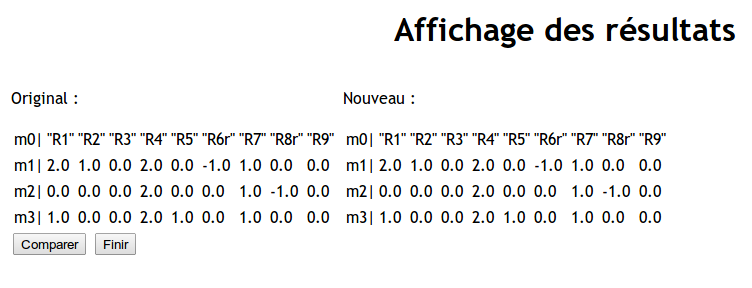
\includegraphics[width=0.90\textwidth]{results_compare.png} 
         \end{minipage}}
        \caption{compare}
          \label{comparaison}
      \end{center}   
\end{figure}

Une fois toutes ces étapes finie, le résultat est sauvegardé dans la variable \emph{compare} pour le cas ou l'utilisateur voudrait comparer son résultat un autre (avec des choix différents d'options, de nouvelles règles, \dots).\\

L'utilisateur a le choix de terminer ses calculs ou de comparer le résultat obtenu. Pour cela, deux boutons \emph{comparer} et \emph{finir} lui permette de retourner à l'écran d'accueil, à la différence près que \emph{comparer} fait appel a la fonction \emph{compare()}  qui conserve en mémoire grace à une variable de session PHP \emph{isCompared} que l'utilisateur veut comparer son résultat et redirige l'utilisateur tandis que l'autre, \emph{finir} réinitialise cette m\^eme variable.


\chapter{Difficultés rencontrées et améliorations à apporter}
Suivant le navigateur utilisé, la récupération des fichiers par la fonction \emph{ move\_uploaded\_file()} ne fournit pas le m\^eme résultats, en particulier le dossier récupérant les fichiers.
 De plus, il semblerait que les variables permettant de récupérer les fichiers \emph{\$FILES} ne fonctionne pas sur toutes les configurations. Jusqu'à présent, nous n'avons pas compris quel facteur influençait l'utilisation de ces variables et n'avons pas pu exécuter regEfmTool depuis l'interface sur toutes les machines.
Les variables de sessions PHP étant propre au langage PHP, nous avons du parfois utiliser les cookies, en particulier lorsque certaines valeurs devaient \^etre sauvegardées depuis un script \emph{JavaScript}. Cela provoque l'utilisation de ces deux types de variables ce qui n'est pas très uniforme.
L'affichage des résultats n'a été fait que superficiellement, d'où la présence de \emph{mode élémentaire 0} devant les noms de réactions ou encore un simple affichage en tableau des résultats brut, indiquant la présence des réactions avec une valeur à 0. l'amélioration de cette partie ne devant pas être trop gourmande en temps mériterait d'\^etre modifiée.
L'utilisation de regEfmTool depuis l'interface que nous avons créée dépend de la configuration du serveur web installé sur la machine. Dans notre cas les tests étaient fait sous \emph{apache2} sur nos machines personnelles, la configuration du serveur sur les machines du \emph{CREMI} étant trop restrictives, il nous était impossible d'exécuter le logiciel..

\chapter*{Conclusion}
\addcontentsline{toc}{chapter}{Conclusion}
Le but de ce projet été de réaliser une interface graphique pour le logiciel de calculs de modes élémentaire \emph{regEfmTool}. L'interface réalisée se présente sous la forme de pages \emph{Web}. Elle permet d'utiliser \emph{regEfmTool} sans avoir à passer par un terminal et permet la création de tous les fichiers d'entrée nécessaire au fonctionnement de ce logiciel.
Elle permet également la création de réseaux au formats \emph{DAT} ce qui permet une édition des réseaux pour le logiciel \emph{Metatool} pour permettre une comparaison des résultats de calculs de modes élémentaire.\\

Ce projet nous a permis de nous familiariser avec les langages propre au communications et protocoles \emph{WEB}, et également de mesurer l'importance d'une bonne gestion d'un travail en équipe aussi bien au niveau de la répartition des taches que de la mise en commun du travail éffectué.
Conclusion ...

\bibliographystyle{unsrt}
\bibliography{rapport}


\end{document}